\subsubsection{Object Adapter}
L'utilizzo della libreria di Freeling, per il pos-tagging, ha richiesto la creazione di un Adapter nella variante Object Adapter per poter adattare le funzionalità strettamente necessarie.
\begin{figure}[H]
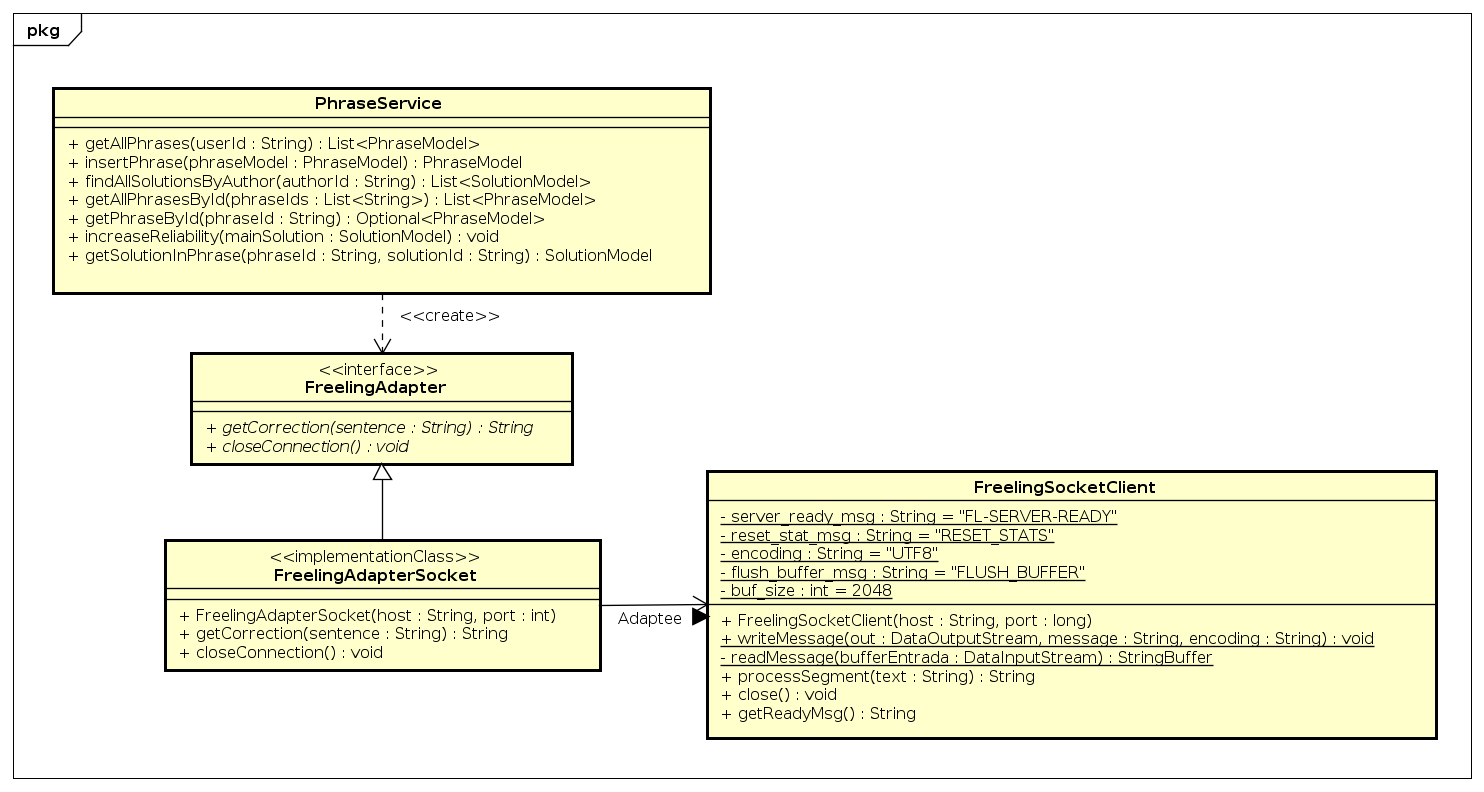
\includegraphics[width=17cm]{img/Adapter.png} 
\caption{Diagramma delle classi Adapter}
\end{figure}
La classe FreelingSocketClient viene fornita dai creatori della libreria e si occupa di realizzare la connessione con il server Freeling scritto in C++.
\subsubsection{Controller - Service - Repository - Model}
L'architettura realizzata all'interno di Spring Web consta nella presenza di:
\begin{itemize}
\item \textbf{Controller}: un a cui è delegato il compito di gestire le richieste provenienti dalla parte frontend e alla cattura delle eccezioni;
\item \textbf{Service}: realizzano la business-logic;
\item \textbf{Repository}: realizzano il layer di persistenza gestendo la base di dati;
\item \textbf{Model}: rappresentano oggetti  Plain Old Java Object, un'istanza di un model rappresenta un documento di una collezione.
\end{itemize}
\begin{figure}[H]
\centering
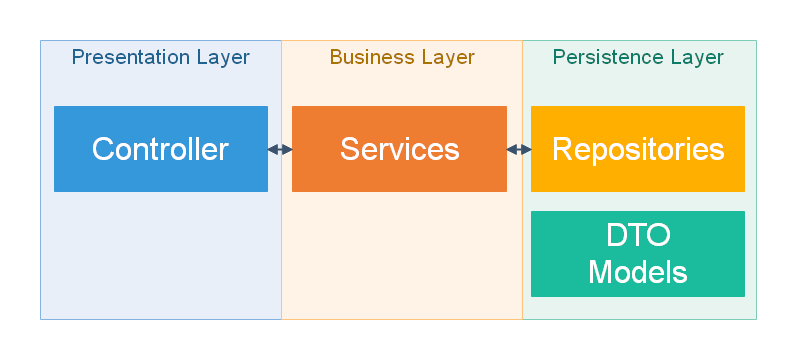
\includegraphics[width=14cm]{img/springArch.png}
\caption{Scherma generale architettura in Spring}
\end{figure}

\subsection{Data Transfer Object}
Le classi Helper rappresentano Data Transfer Object (DTO), vengono utilizzate dalla classe \texttt{Controller.java} per fornire un oggetto per il trasferimento dati dalla frontend senza ricorrere a JSON troppo complessi.

\subsubsection{Builder}
I model sono dotati ognuno di un builder, tale classe interna non è codificata ma realizzata tramite un plugin denominato lambok.